\item \textbf{{[}ALVL/9597/2019/P2/Q1{]} }

A supermarket chain wants to encourage customers to return to its
store. They operate a scheme of rewards for customers based on how
much they spend over a period of time.

Customers are issued with a card that is readable by a Point of Sale
(POS) terminal. When a customer provides their card at the checkout,
the system identifies them and stores the products they purchased
and how much they spent.

Currently the only use of this data is to issue the customer with
vouchers every three months. Vouchers have a value based on the total
amount the customer has spent during the previous three months. The
vouchers can only be used in part payment for goods bought in the
supermarket.

The supermarket managers want to make more use of the customer purchase
data. They hire a software development company to produce software
that will implement new uses of the data.

Software developers have skills in developing software. The supermarket
managers have in depth knowledge of their business. At first, software
developers will have little knowledge of the business.
\begin{enumerate}
\item Explain how the supermarket managers can communicate to the software
developers what they require. \hfill{}{[}2{]}
\item Before designing the new software, the software developers need to
understand the content and structure of the customer purchase data.
Give two methods that can be used for this task, justifying the use
of each. \hfill{}{[}4{]}
\item Once the analysis phase has been completed, describe what decisions
software developers need to make before coding can begin. \hfill{}{[}6{]}
\end{enumerate}
The work to implement new uses of the customer data needs to be managed.
The following Program Evaluation and Review Technique (PERT) chart
is used as a management tool.

Time is measured in weeks. 
\begin{center}
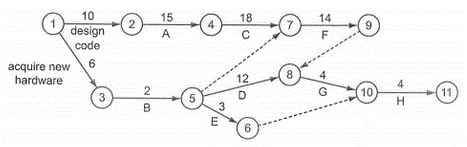
\includegraphics[width=0.7\paperwidth]{C:/Users/Admin/Desktop/Github/question_bank/LyX/static/img/9597-ALVL-2014-P2-Q1}
\par\end{center}
\begin{enumerate}
\item[(d)]  Each activity indicated by a dashed line on the PERT chart is a
dummy activity.
\begin{enumerate}
\item Explain the nature and purpose of a dummy activity.\hfill{} {[}2{]}
\item Each of the following activities matches one of the labels A-H on
the chart.
\begin{itemize}
\item write user documentation 
\item train users 
\item write code 
\item convert files
\item test code 
\item end-user testing 
\item test system 
\item install new hardware
\end{itemize}
Copy and complete the following table, 
\begin{center}
\begin{tabular}{|c|>{\centering}p{0.5\columnwidth}|}
\hline 
Label & Activity\tabularnewline
\hline 
A & \tabularnewline
\hline 
B & \tabularnewline
\hline 
C & \tabularnewline
\hline 
D & \tabularnewline
\hline 
E & \tabularnewline
\hline 
F & \tabularnewline
\hline 
G & \tabularnewline
\hline 
H & \tabularnewline
\hline 
\end{tabular}
\par\end{center}

\hfill{}{[}4{]}
\item Explain the significance of the dummy activity that leads into event
8. \hfill{}{[}3{]}
\end{enumerate}
\item[(e)]  From the PERT chart:
\begin{enumerate}
\item State the critical path.\hfill{} {[}1{]}
\item State the minimum time in which the new software can be developed
and implemented.\hfill{} {[}1{]}
\item The chart omits an activity: \textbf{write technical documentation}.
State a starting point and a finishing point for this activity. Justify
your choices. \hfill{}{[}4{]}
\end{enumerate}
\end{enumerate}
Management staff can already access the company network remotely for
other software applications. Management are to be given the facility
to access, and interact with, the customer data Via the company LAN.
However, a decision is made not to allow access to the customer data
remotely for this updated system.
\begin{enumerate}
\item[(f)]  Describe \textbf{two} methods which can be used to ensure that there
is no remote access to customer data by management staff. \hfill{}{[}4{]}
\end{enumerate}
ln the new system, customers will have access to information through
a web browser. Each customer will be able to see some information
about their purchase history.
\begin{enumerate}
\item[(g)]  Explain what software needs to be developed to provide this customer
facility. \hfill{}{[}5{]}
\item[(h)]  One of the software developers has the task of ensuring that social
issues are considered. This developer has to document these issues. 

Describe \textbf{two} issues that might be in the document with regard
to customers accessing their data. \hfill{}{[}4{]}
\end{enumerate}